\documentclass[12pt]{article}
\usepackage[utf8]{inputenc}
\usepackage{graphicx} 
\usepackage{fancyhdr}
\usepackage{colortbl}
\usepackage{geometry}
\usepackage{xcolor}
\usepackage{float}
\usepackage{booktabs}
\usepackage[english]{babel}
\linespread{1.25} 
\setlength{\parindent}{0pt} 
\setlength{\parskip}{1em}
\renewcommand{\headrulewidth}{0pt} 
\geometry{legalpaper, portrait, margin=1in}
\setlength{\headheight}{14.49998pt}

\begin{document}
\begin{titlepage}
   \begin{center}
        \vspace*{5cm}

        \Huge{R Hidden Curriculum Assignment}

        \vspace{0.5cm}
        \LARGE{Analyzing 2002 Incarcerations by Race and Gender}
            
        \vspace{3 cm}
        \Large{Alice Kemp}
       
        \vspace{3 cm}
        \Large{February 18th, 2022}
        
        \vspace{0.25 cm}
        \Large{The University of Texas at Austin}

        \vspace{0.25 cm}
        \Large{ECO395M}
       

       \vfill
    \end{center}
\end{titlepage}

\setcounter{page}{2}
\pagestyle{fancy}
\fancyhf{}
\rhead{\thepage}

\section*{Overview}
In this report, I seek to assess the relationship, if any, between race, gender, and length of incarceration for individuals incarcerated for at least one month during the 12-month period studied in the year 2002.  

\section*{Methodology}
Data was collected from the National Longitudinal Survey (NLS), sponsored by the U.S. Bureau of Labor Statistics (BLS). The specific variable of interest analyzed was monthly incarceration status by race and gender in 2002, selected from the National Longitudinal Survey of Youth 1997 (NLSY97) cohort.
The data was then restricted to exclude skipped individual responses and individuals already incarcerated and further filtered to remove individuals with null responses for the duration of the 12-month time frame and those who were never incarcerated during this period.  

\section*{Analysis}
To visualize the differences in average months of incarceration in 2002 across race and gender classifications, the filtered data was first aggregated by race and gender. Then, average length of incarceration, measured in months, was calculated for each group. The averages were then plotted in a mixed bar plot with race classification and gender on the x-axis and mean incarceration length on the y-axis (Figure 1). We found that average incarceration length diverged the most across genders for Black individuals, or approximately 8 months for males and 2.7 months for females. These also were the highest and lowest average incarceration lengths across all groups. The least divergent race was Hispanics, with males averaging 0.6 months longer than females. For mixed race individuals, data points were limited (an issue to be expanded upon further) with no data points for males and only one data point yielding a 6 month average for females. Finally, for non-Blacks/non-Hispanics, males averaged 1.44 months longer in incarceration than females. 

\begin{figure}[H]
    \begin{center}
        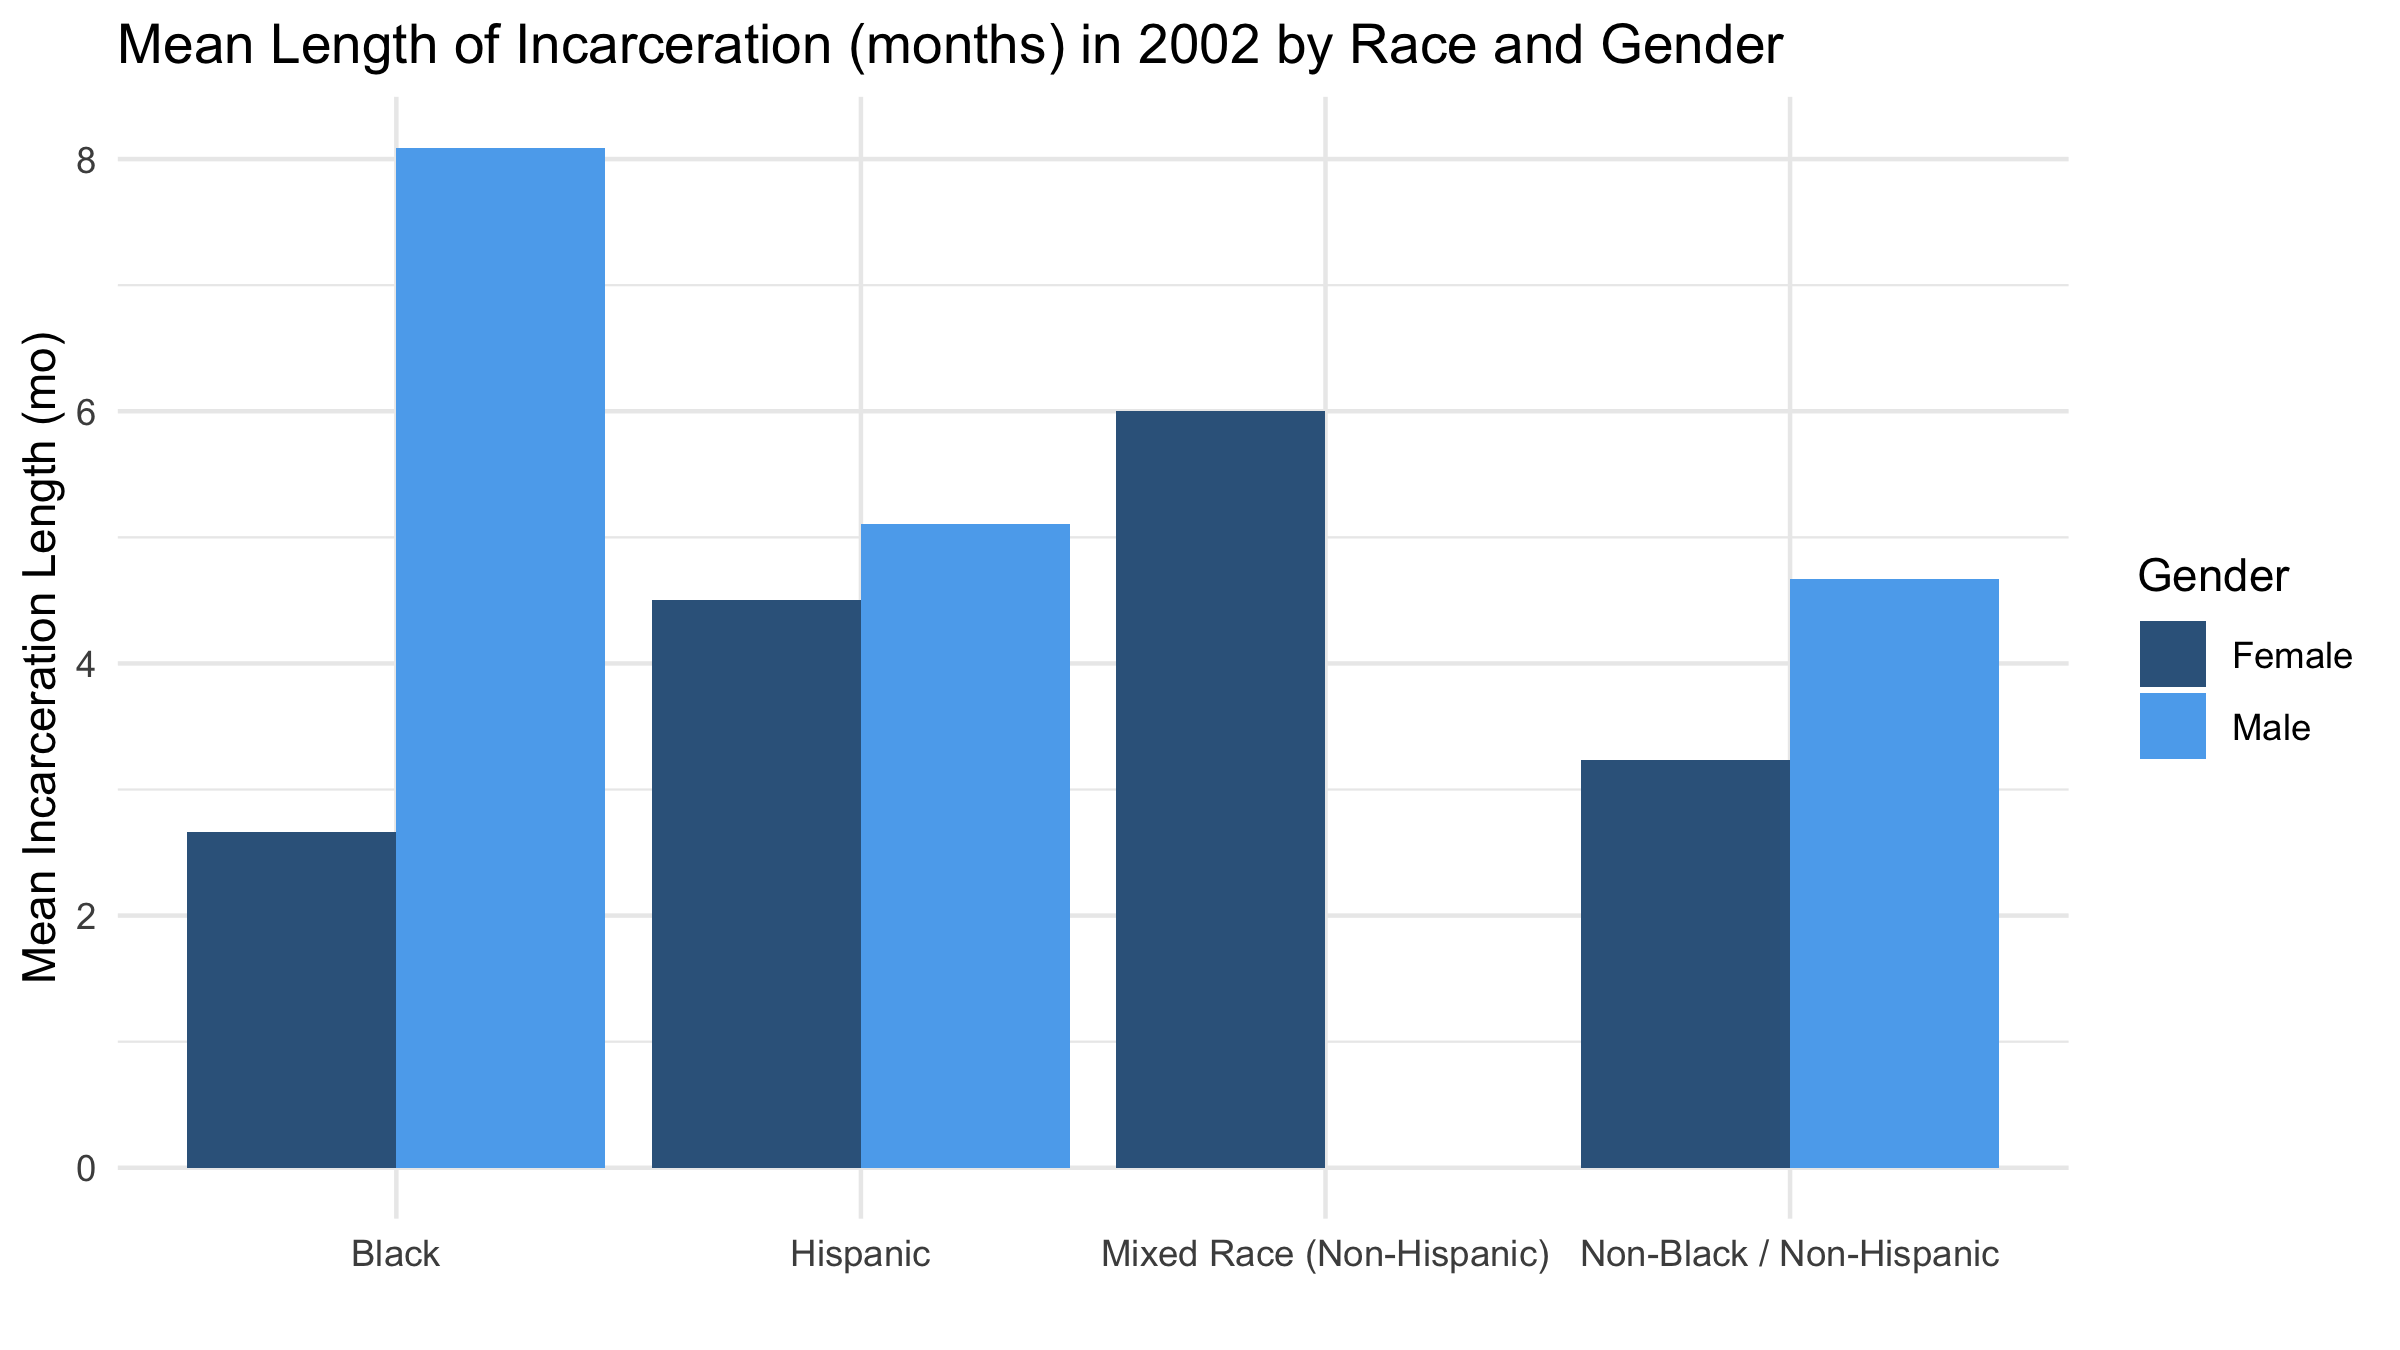
\includegraphics[width=.85\textwidth]{incarcerations_by_racegender}
    \end{center}
    \caption{Mean incarceration length in 2002 by Race and Gender}
    \label{fig:graph}
\end{figure}


\begin{table}[H]
\begin{table}[H]

\caption{\label{tab:tab:summarystats}Mean incarceration length (months) in 2002 by Race and Gender}
\centering
\begin{tabular}[t]{lrrrr}
\toprule
Gender & Black & Hispanic & Mixed Race Non Hispanic & Non Black Non Hispanic\\
\midrule
\cellcolor{gray!6}{Female} & \cellcolor{gray!6}{2.666667} & \cellcolor{gray!6}{4.500000} & \cellcolor{gray!6}{6} & \cellcolor{gray!6}{3.230769}\\
Male & 8.090909 & 5.103448 & NA & 4.666667\\
\bottomrule
\end{tabular}
\end{table}

\end{table}

\section*{Model}
To model the statistical relationship between race, gender, and incarceration time, a linear OLS regression was run using Hispanic, Mixed Race (Non-Hispanic), Non-Black/Non-Hispanic, and Male features, with the constant term equating to the Black Female coefficient. The regression (Table 2) shows that Hispanic females have, on average, an expected incarceration that is 2.3 months shorter in 2002 than Black females - approximately 2.8 months long, holding all else fixed. Similarly, Non-Black/Non-Hispanic females have an expected incarceration that is approximately 2.9 months shorter than Black females, or approximately 2.2 months long, holding all else fixed. Mixed Race (Non-Hispanic) females have an expected incarceration of 6 months, or 0.8 months longer than Black females, holding all else fixed. Finally, males have an expected incarceration that is 2.6 months longer than Black females on average, holding all else fixed. 

According to the model, none of the features of interest are statistically significant. Therefore, we cannot say with confidence that these relationships exist and are not due to random variation in the data. Furthermore, the sample size after filtering included 178 individuals, with certain race and gender classifications including only a few or zero individuals, in particular the Mixed Race (Non-Hispanic) group. Thus, a larger sample size would allow repeated analysis to establish any statistically significant effects. 

\begin{table}[H]

% Table created by stargazer v.5.2.2 by Marek Hlavac, Harvard University. E-mail: hlavac at fas.harvard.edu
% Date and time: Wed, Feb 16, 2022 - 13:46:09
\begin{table}[!htbp] \centering 
  \caption{Regression Output. Omitted category is Black Females.} 
  \label{tab:regression} 
\begin{tabular}{@{\extracolsep{5pt}}lc} 
\\[-1.8ex]\hline 
\hline \\[-1.8ex] 
 & \multicolumn{1}{c}{\textit{Dependent variable:}} \\ 
\cline{2-2} 
\\[-1.8ex] & Length of Incarceration in 2002 \\ 
\hline \\[-1.8ex] 
 Hispanic & $-$2.306 \\ 
  &  \\ 
  & \\ 
 Mixed Race (Non-Hispanic) & 0.857 \\ 
  &  \\ 
  & \\ 
 Non-Black / Non-Hispanic & $-$2.859 \\ 
  &  \\ 
  & \\ 
 Male & 2.610 \\ 
  &  \\ 
  & \\ 
 Constant & 5.143 \\ 
  &  \\ 
  & \\ 
\hline \\[-1.8ex] 
Observations & 178 \\ 
R$^{2}$ & 0.161 \\ 
Adjusted R$^{2}$ & 0.142 \\ 
Residual Std. Error & 3.946 (df = 173) \\ 
F Statistic & 8.302$^{***}$ (df = 4; 173) \\ 
\hline 
\hline \\[-1.8ex] 
\textit{Note:}  & \multicolumn{1}{r}{$^{*}$p$<$0.1; $^{**}$p$<$0.05; $^{***}$p$<$0.01} \\ 
\end{tabular} 
\end{table} 

\end{table}

\end{document}
